\documentclass[11pt,reqno]{amsart}
\usepackage[T1]{fontenc}
\usepackage[utf8]{inputenc}
\usepackage{lmodern,microtype,mathtools,amssymb,booktabs,longtable,array,enumitem}
\usepackage[a4paper,margin=1.05in]{geometry}
\usepackage{tikz}
\usetikzlibrary{arrows.meta,positioning,calc}
\usepackage{xcolor}
\definecolor{linkblue}{RGB}{24,70,78}
\usepackage[colorlinks=true,linkcolor=linkblue,citecolor=linkblue,urlcolor=linkblue,pdfencoding=auto]{hyperref}
\hypersetup{pdftitle={Compiling Stochastic Chemical Trajectories with Elementary Reactions},pdfauthor={Harjas Sandhu}}
\newtheorem{theorem}{Theorem}[section]
\newtheorem{lemma}[theorem]{Lemma}
\newtheorem{proposition}[theorem]{Proposition}
\newtheorem{corollary}[theorem]{Corollary}
\theoremstyle{definition}
\newtheorem{definition}[theorem]{Definition}
\newtheorem{example}[theorem]{Example}
\theoremstyle{remark}
\newtheorem{remark}[theorem]{Remark}
\newcommand{\N}{\mathbb N}
\newcommand{\R}{\mathbb R}
\newcommand{\E}{\mathbb E}
\newcommand{\Prob}{\mathbb P}
\newcommand{\TV}{d_{\mathrm{TV}}}
\newcommand{\Law}{\mathcal L}
\newcommand{\hid}{\dagger}
\newcommand{\ff}[2]{(#1)_{#2}}
\newcommand{\one}{\mathbf 1}
\newcommand{\norm}[1]{\lVert#1\rVert}
\newcommand{\abs}[1]{\lvert#1\rvert}
\DeclareMathOperator{\Pois}{Pois}
\DeclareMathOperator{\Obs}{Obs}
\setlist[itemize]{leftmargin=1.6em,itemsep=.35em,topsep=.5em}
\setlist[enumerate]{leftmargin=2em,itemsep=.35em,topsep=.5em}
\setcounter{tocdepth}{1}
\allowdisplaybreaks[2]

\begin{document}
\title[Elementary stochastic trajectory compilation]{Compiling Stochastic Chemical Trajectories\\ with Elementary Reactions}
\author{Harjas Sandhu}
\address{The University of Queensland, Brisbane, Australia}
\email{harjas.sandhu@student.uq.edu.au}
\date{13 November 2026}
\subjclass[2020]{60J27, 92C42, 68Q05, 92E20}
\keywords{Stochastic reaction networks, elementary reactions, marked paths, total variation, chemical compilation, predictable perturbations, detailed balance}
\begin{abstract}
We construct elementary mass-action networks that approximate the complete
labelled trajectories of finite stochastic reaction lists of variable dimension
and order. The input supplies a positive integer population weight and a global
upper bound on its drift. The compiled structure and decoder depend only on the
reaction list; all decoder columns are nonzero, and initialization uses exactly
zero auxiliary molecules. Directed reachability is preserved for every fine
state. One constant slowdown and rational coefficients give finite-horizon
marked-path total-variation accuracy under arbitrary predictable coordinated
multiplicative rate errors. Exact rescaled event times, original null labels and
parallel labels are retained. A bounded pending-reaction credit and pathwise
counting identities pay population and every fine firing throughout the actual
untruncated run. Compiler bit costs and charged numerical physical costs have
universal polynomial bounds, with reaction order included in the input.
A separate paired construction supplies exact nominal detailed balance,
conservation and the same timed-path guarantee for conservative reversible
inputs with prescribed rational activities. The results concern ideal
mass-action models; they do not construct molecular synthesis pathways or
establish practical efficiency.
\end{abstract}
\maketitle
\tableofcontents
\section{Introduction}
A stochastic chemical model can prescribe a reaction involving many molecules
at once. An elementary implementation must instead assemble, transform and
release those molecules through small steps. The intermediate reactions take
time and create additional random events. Consequently, preserving a
reaction's net stoichiometry does not establish that the implementation has the
same observable dynamics.

The question here is quantitative: can one replace a whole finite reaction
list by reactions involving at most two molecules on each side, while
approximating its complete timed, labelled trajectory and paying for all the
intermediate work? We permit reaction order, dimension and initial populations
to vary. The original system may be open, with no stationary distribution or
conservation law. Its supplied population certificate is only a global upper
drift bound.

\subsection{The contribution}
Theorem~\ref{thm:open} gives such a compiler. Its species, channel structure and
integer decoder depend only on the labelled stoichiometric list. Numerical
rates, one slowdown and an error tolerance are then chosen from the full input.
The initial auxiliary population is exactly zero. Every auxiliary molecule
represents a nonempty multiset of original molecules, so there is no initially
supplied controller or zero-payload fuel species.

Two conclusions are especially important. First, the graph statement holds
from \emph{every} fine state: directed reachability and communicating classes
are exactly reflected by the decoder. Second, accuracy and actual work are
uniform over predictable rate faults that may observe and use the entire fine
history. The physical chain keeps running on rare excursions. Its population
and all-event costs are bounded for every physical time, not just on the event
where a finite-horizon comparison succeeds.

The core global estimate uses \emph{pending molecules}. Each contains the true
source payload of a reaction that may complete. Sparse binary collisions return
pending molecules to their source representatives. A bounded credit assigns to
each pending molecule an upper estimate of its chance to complete before
returning. Its drift controls all completions, including null and parallel
marks. Exact counting identities then pay even the rapid, unsuccessful assembly
cycles. This mechanism is distinct from the finite-fibre averaging used for
accuracy.

Theorem~\ref{thm:balanced} gives a separate conservative, nominally
detailed-balanced compiler. It uses paired source chains, different weights and
different central rates. Conservation supplies its global work bound. The
irreversible collision returns of the main construction are absent. Thus the
balanced theorem is an additional construction, not a detailed-balance claim
about the open compiler.

\subsection{Relation to previous methods}
Chemical programming and experimental molecular controllers are established
subjects; programmable DNA controllers have been demonstrated by Chen et
al.~\cite{Chen2013}. The present theorem is a statement about a specified
stochastic mass-action model and its quantitative compilation contract.

Intermediate-species elimination and stochastic averaging are also established.
Hoessly--Wiuf~\cite[Assumption~2 and Theorem~4.1]{HW2021} prove compact-time
state-probability reduction under their non-interacting-species, fast-return and
finite-closed-set hypotheses. Their Section~4.2 gives a time-dependent version
with stated regularity. Here the target can have unbounded state space; the
output retains the entire marked path, with finite rates, quantitative work
bounds and history-dependent perturbations. We prove the required path estimate
rather than infer it from convergence of marginals.

The factorial fibre law used below is standard product-form algebra.
Anderson--Craciun--Kurtz~\cite[Theorem~4.1 and Section~4.2]{ACK2010} describe
Poisson invariant laws and the relation between chemical detailed balance and
stochastic reversibility. We verify the finite-fibre identities directly.
Spatial detailed balance requires further conditions: Zhang--Isaacson's
bounded-domain analysis~\cite[Section~III, Theorem~III.1]{ZI2022} treats reversible
association--dissociation fluxes and product placement. Such spatial conditions
are not consequences of a kinetic graph lift. Appendix~\ref{app:literature}
records the precise uses of these comparisons.

The contribution is the joint constructive guarantee: variable-order elementary
lowering, all-state graph fidelity, canonical initialization, exact-time marked
path approximation, predictable-fault robustness and a complete numerical and
binary cost account. No claim of historical firstness is needed for that
statement.

\subsection{Conceptual overview}
Figure~\ref{fig:pipeline} separates the actual operation from its analytical
comparison. A reaction first assembles its source in a private chain. A pending
species then either returns or completes into a private product chain. The
physical system runs all these reactions autonomously with constant nominal
coefficients. Observation applies a fixed decoder and hides only auxiliary
labels.

For the proof, a weighted cutoff makes the relevant fibres finite. Hidden
release estimates yield a uniform canonical atom, which gives a mixing
integral. An independent proposal clock, used only in the coupling, compares
full marked paths at their actual event times. The supplied drift bound controls
the original process's exit probability. Independently, the pending credit
controls actual work everywhere, including beyond that cutoff.

\begin{figure}[tb]
\centering
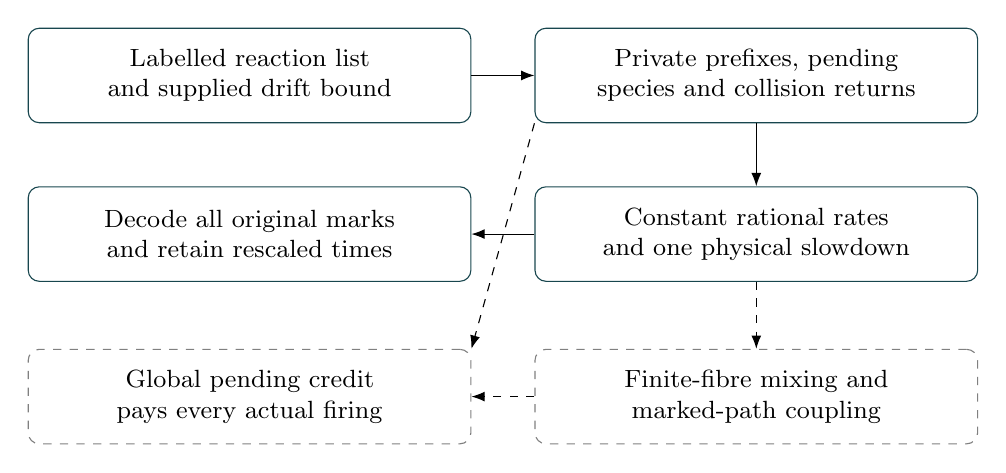
\begin{tikzpicture}[>=Latex,font=\small,
 box/.style={draw=linkblue,rounded corners,align=center,text width=5.2cm,minimum height=1.2cm,inner sep=6pt},
 proof/.style={draw=gray,dashed,rounded corners,align=center,text width=5.2cm,minimum height=1.2cm,inner sep=6pt}]
\node[box] (input) {Labelled reaction list\\and supplied drift bound};
\node[box,right=0.8cm of input] (fine) {Private prefixes, pending\\species and collision returns};
\node[box,below=0.8cm of fine] (run) {Constant rational rates\\and one physical slowdown};
\node[box,left=0.8cm of run] (out) {Decode all original marks\\and retain rescaled times};
\draw[->] (input)--(fine);\draw[->] (fine)--(run);\draw[->] (run)--(out);
\node[proof,below=0.85cm of out] (tail) {Global pending credit\\pays every actual firing};
\node[proof,right=0.8cm of tail] (couple) {Finite-fibre mixing and\\marked-path coupling};
\draw[->,dashed] (fine.south west)--(tail.north east);
\draw[->,dashed] (run)--(couple);
\draw[->,dashed] (couple)--(tail);
\end{tikzpicture}
\caption{The upper four boxes describe the emitted operation. Dashed boxes
are proof mechanisms. No cutoff, equilibrium sampler, proposal clock or
externally performed reset is part of the physical network.}
\label{fig:pipeline}
\end{figure}

The reading order is as follows. Section~\ref{sec:model} states the exact
contract. Sections~\ref{sec:network}--\ref{sec:global} construct the network and
pay its whole run. Sections~\ref{sec:fibre}--\ref{sec:path} prove timed-path
accuracy. Section~\ref{sec:compiler} and Appendix~\ref{app:resources} establish
the compiler and resource bounds. Section~\ref{sec:examples} gives examples,
and Section~\ref{sec:balanced} proves the balanced conservative interface.

\section{Model, observation and main theorem}\label{sec:model}
\subsection{Input and the drift promise}
Let $\N=\{0,1,\ldots\}$. A finite labelled reaction list on $d$ declared species
$A_1,\ldots,A_d$ is
\[
 \mathcal R=((y_r,z_r):r=1,\ldots,m),\qquad y_r,z_r\in\N^d.
\]
Each complex is supplied as an explicitly expanded list of molecule indices;
its order is therefore paid in the input length. Empty, null and parallel
reactions are permitted. Empty sums and maxima are taken as zero. Put
\[
 q_r=|y_r|_1,\quad q'_r=|z_r|_1,\quad
 D=\max\bigl(1,\max_r(q_r\vee q'_r)\bigr).
\]
For $x,y\in\N^d$, write
\[
 (x)_y=\prod_i x_i(x_i-1)\cdots(x_i-y_i+1),
\]
with $(x)_0=1$ and $(x)_y=0$ unless $x\ge y$. All propensities are at unit
volume, with no additional symmetry factors. The original marked intensity is
\begin{equation}\label{eq:original-rate}
 \lambda_r(x)=k_r(x)_{y_r},\qquad 0<k_r\le1,
\end{equation}
where the $k_r$ are rational. A firing of label $r$ changes $x$ to
$x-y_r+z_r$, even when this equals $x$.

The remaining input consists of binary initial counts $x_0$, positive integer
weights $\omega_i$, and rationals $A\ge0$, $\tau>0$, $0<\epsilon<1/8$.
Set $N(x)=\omega\cdot x$ and $N_0=N(x_0)$. The admission promise is
\begin{equation}\label{eq:drift-promise}
 LN(x)=\sum_r k_r(x)_{y_r}\,\omega\cdot(z_r-y_r)\le A
 \quad\text{for every }x\in\N^d.
\end{equation}
The compiler is not required to decide this inequality. In particular, a
certificate is supplied as a mathematical promise, not discovered by a
normalizer, optimization or state-space oracle.

\subsection{Marked paths and physical time}
On reference time $[0,\tau]$, a complete original marked path is its initial
state and the finite sequence
\begin{equation}\label{eq:marked-record}
 (t_j,r_j,x_j)_{j=1}^{J},\qquad
 0<t_1<\cdots<t_J\le\tau,
\end{equation}
where $x_j$ is the state just after the event. It retains a null event even
when $x_j=x_{j-1}$, and distinguishes labels with identical increments. This
record determines the piecewise constant state path and its final waiting
interval. We use the usual Borel structure on the disjoint union of these
finite-sequence spaces. For laws $\mu,\nu$, total variation means
$\TV(\mu,\nu)=\sup_E|\mu(E)-\nu(E)|$.

A fine network has $s$ species, elementary channels
$\alpha_e\to\beta_e$ with $|\alpha_e|_1,|\beta_e|_1\le2$, an integer decoder
$P\in\N^{d\times s}$, and a map $\ell(e)\in\{1,\ldots,m\}\cup\{\hid\}$.
The symbol $\hid$ denotes a hidden mark. Canonical initialization is
$j(x)=(x,0)$, and the original columns of $P$ are the identity.

The emitted physical coefficients are constant rationals $c_e$. At physical
time $s$, the actual channel intensity is
\begin{equation}\label{eq:fault-rate}
 c_e a_e(s)(Z_{s-})_{\alpha_e},\qquad
 1-\delta\le a_e(s)\le1+\delta.
\end{equation}
The multipliers are arbitrary real predictable processes for a filtration in
which the driving Poisson noise has independent future increments. They may
coordinate using all prior fine states, hidden and observed marks, null and
parallel events, and external randomness. No continuity or switching bound is
assumed. They are faults, not chosen controls.

Given one slowdown $H\ge1$, the observation $\Obs_{H,\ell}(Z)$ keeps $PZ_0$
and every fine firing with $\ell(e)\ne\hid$, with physical event time divided
by $H$, original label $\ell(e)$ and decoded post-event state. The observed
physical interval is $[0,H\tau]$. We always use $t$ for reference time and $s$
for physical time.

\begin{center}
\small
\begin{tabular}{p{.20\linewidth}p{.70\linewidth}}
\toprule
Symbol & Meaning\\\midrule
$x$, $X_t$ & Decoded/original state and target process in reference time.\\
$u$, $Z_s$ & Fine state and actual process in physical time.\\
$n(u)$, $V(u)$, $N(Pu)$ & Fine count $|u|_1$, unweighted decoded count $|Pu|_1$, and weighted decoded count.\\
$P$, $j$, $\ell$ & Fixed decoder, zero-auxiliary encoding and label map.\\
$K$, $Q$, $\eta$, $H$, $\delta$ & Chosen rational rate parameters, slowdown and fault tolerance.\\
$B$, $\Gamma_B$, $W$ & Analytical cutoff, charged activity envelope and numerical charge.\\
$q(x)$, $\nu_x$, $I$ & Proof-only partition polynomial, fibre law and mixing integral.\\
\bottomrule
\end{tabular}
\end{center}
The physical count, decoded count and weighted decoded count are not
interchangeable. Chosen parameters and proof-only variables are distinguished
in the guide above.

\subsection{Numerical and binary resources}
Let $L$ be the complete binary length, including the species declarations,
expanded complexes, counts, weights and all rational data. Define
\begin{align}
 B&=1+\left\lceil\frac{32(N_0+A\tau+1)}{\epsilon}\right\rceil,
 & U&=1+B,\label{eq:cutoff}\\
 \Gamma_B&=2+m+\sum_r k_r(1+B)^{q_r},\label{eq:gamma}\\
 W&=2+d+m+D+\sum_i\omega_i+N_0+A+\tau+\tau^{-1}
       +\epsilon^{-1}+\Gamma_B+\sum_r k_r^{-1}.\label{eq:W}
\end{align}
$B$ is an analytical cutoff, not a reflecting wall. $\Gamma_B$ is a computed
rational activity envelope, not an oracle. Its binary length is polynomial in
$L$, although its numerical magnitude may grow rapidly with order and
population. The binary cost is charged in $L$; physical numerical costs are
charged in $W$.

\newpage
\begin{theorem}[Open elementary trajectory compiler]\label{thm:open}
There is a total deterministic algorithm with the following properties.
For every labelled list $\mathcal R$, it constructs a fine species and channel
structure, $P$ and $\ell$ depending only on $\mathcal R$. Every decoder column
is nonzero. Hidden channels preserve $P$, and every observed channel labelled
$r$ realizes an enabled original edge. For every pair of fine states,
\begin{equation}\label{eq:graph-theorem}
 u\leadsto v\quad\Longleftrightarrow\quad Pu\leadsto Pv.
\end{equation}
Its communicating classes are exactly $P^{-1}(\mathcal C)$ as $\mathcal C$
ranges over the original communicating classes.
For every numerical input above, the algorithm emits positive rational
$c_e\le1$, $H\ge1$ and $0<\delta\le1/2$. If
\eqref{eq:drift-promise} holds, then under \emph{every} fault family
\eqref{eq:fault-rate}, the fine process from $j(x_0)$ is nonexplosive for all
physical times and
\begin{equation}\label{eq:main-TV}
 \TV\bigl(\Law(\Obs_{H,\ell}(Z)),\Law(X\text{ marked on }[0,\tau])\bigr)
 \le\epsilon.
\end{equation}
The same emitted output works for every such family. With
$C=2^{4096}$ and $p=256$, binary work, memory and total output bits are at most
$C(1+L)^p$, while
\begin{equation}\label{eq:main-numeric}
 H,\ H\tau,\ \delta^{-1},\ \max_e c_e^{-1}\ \le C W^p.
\end{equation}
Writing $F_{\rm all}(s)$ for all actual fine firings, including hidden and null
firings, for every physical $s\ge0$,
\begin{align}
 \E\sup_{0\le v\le s}(1+|Z_v|_1)&\le CW^p(1+s),\label{eq:main-pop}\\
 \E F_{\rm all}(s)&\le CW^p(1+s)^2,\label{eq:main-firing}\\
 \E F_{\rm all}(H\tau)&\le CW^p.\label{eq:main-horizon}
\end{align}
The structure and graph assertions do not depend on the drift promise.
The algorithm terminates on nonadmitted inputs as well.
\end{theorem}

The bounds are explicit sufficient bounds, not optimal exponents or measured
performance. All labelled events and waiting times occur in the physical
network. The conclusion approximates a path \emph{law}; it is not an equality of
laws or an exact-sampling claim.

\subsection{A preliminary consequence of the promise}
\begin{lemma}[Target escape and nonexplosion]\label{lem:target-tail}
The original marked process is nonexplosive and, for $b>N_0$,
\begin{equation}\label{eq:target-tail}
 \Prob\left\{\sup_{t\le\tau}N(X_t)\ge b\right\}
 \le\frac{N_0+A\tau}{b}.
\end{equation}
\end{lemma}
\begin{proof}
Stop the minimal process at its first entrance into $N\ge b$. Below that level
there are finitely many original states, and every marked rate is bounded.
The finite reaction list also bounds the overshoot of $N$. Localized Dynkin's
formula therefore gives
$\E N(X_{t\wedge\sigma_b})\le N_0+At$. Nonnegativity yields
\eqref{eq:target-tail}. Letting $b\to\infty$ prevents population escape in
finite time. An infinite number of firings with bounded population is
impossible because the total intensity, including null labels, is bounded on
each finite population set. This proves nonexplosion and removes localization.
\end{proof}



\section{The elementary network}\label{sec:network}
\subsection{Private prefixes and true payloads}
Order the explicitly listed molecules of each complex deterministically.
For label $r$, create source-prefix species $S_{r,j}$ for $2\le j\le q_r$,
product-prefix species $T_{r,j}$ for $2\le j\le q'_r$, and a pending species
$C_r$ when $q_r>0$. All these names are private, even when two prefixes have
the same decoded multiset. In particular, a null reaction has separate source
and product chains.

A prefix decodes to its first $j$ original molecules; $PC_r=y_r$. Define the
source representative $s_r$ to be its original species if $q_r=1$, or
$S_{r,q_r}$ otherwise. Define the product representative $t_r$ to be the empty
complex if $q'_r=0$, its original species if $q'_r=1$, or $T_{r,q'_r}$ otherwise.
For any fine species $S$, put $d_S=|PS|_1$. Then
\begin{equation}\label{eq:counts-order}
 1\le d_S\le D,\qquad
 n(u):=|u|_1\le V(u):=|Pu|_1\le N(Pu).
\end{equation}
Thus an auxiliary is a representation of real decoded population, rather than
a free token that disappears under observation.

For an ordered source $A_{i_1}+\cdots+A_{i_q}$, emit the hidden pairs
\begin{equation}\label{eq:prefix-reactions}
 A_{i_1}+A_{i_2}\rightleftarrows S_{r,2},\qquad
 S_{r,j-1}+A_{i_j}\rightleftarrows S_{r,j}\quad(3\le j\le q),
\end{equation}
and analogous hidden product pairs. For $q_r>0$, add a hidden initiation and
return pair, and an observed completion:
\begin{equation}\label{eq:pending-reactions}
 s_r\rightleftarrows C_r,\qquad C_r\xrightarrow{r}t_r.
\end{equation}
For $q_r=0$, the observed channel is $\varnothing\xrightarrow{r}t_r$.
When $t_r=\varnothing$, this includes an actual $\varnothing\to\varnothing$
mark.

Finally, for every nonempty-source label $r$ and \emph{every} fine species $S$,
emit the hidden collision return
\begin{equation}\label{eq:collision}
 C_r+S\longrightarrow s_r+S.
\end{equation}
For $S=C_r$, its source is $2C_r$ and its propensity uses $(u_{C_r})_2$.
The spectator is retained, including when it is another pending molecule.
These reactions preserve the decoder and have at most two molecules on each
side. Their small positive rate is essential for the global estimate.

Writing
\[
 S_{\rm p}=\sum_r(q_r-1)_++\sum_r(q'_r-1)_+,
 \qquad m_+=|\{r:q_r>0\}|,
\]
the numbers of species and directed labelled channels are
\begin{equation}\label{eq:network-size}
 s=d+S_{\rm p}+m_+,\qquad
 m_f=2S_{\rm p}+2m_++m+m_+s.
\end{equation}
The auxiliary populations are all initially zero. This construction uses only
the labelled stoichiometry.

\subsection{Exact directed reachability}
\begin{proposition}\label{prop:graph}
The network satisfies all graph assertions of Theorem~\ref{thm:open}.
\end{proposition}
\begin{proof}
Hidden prefix steps and pending returns preserve the decoder, as does
\eqref{eq:collision}. If a nonempty-source completion can fire, its consumed
$C_r$ carries $y_r$, so $Pu\ge y_r$ and the decoded change is $z_r-y_r$.
The assertion for an empty source is immediate.

From any fine state, first return each pending molecule through its baseline
hidden return and then release every prefix. These unary releases terminate:
they decrease the total number of bonds represented by prefixes. The result
is $j(Pu)$. Every step used has a hidden reverse. Hence
\begin{equation}\label{eq:canonical-connectivity}
 u\longleftrightarrow j(Pu)
 \quad\text{in the hidden graph, for every }u.
\end{equation}
An enabled original edge from $x$ has a lift from $j(x)$: assemble its private
source, enter $C_r$, fire its completion, and release the product. For an empty
source, omit the first two operations. Consequently an original directed path
lifts between canonical encodings. Together with
\eqref{eq:canonical-connectivity}, this proves the reverse implication in
\eqref{eq:graph-theorem}. Projecting a fine path and deleting hidden marks
proves the forward implication. Every fine communicating class is therefore
exactly $P^{-1}(\mathcal C)$ for an original communicating class $\mathcal C$.
The release paths in this proof are graph witnesses, not scheduled physical
operations.
\end{proof}

\subsection{One explicit choice of rates}
For $m>0$, abbreviate $\Gamma=\Gamma_B$ and $k_* =\min_r k_r$. Set
\begin{align}
 C_{\rm f}&=16(D+1)^2\bigl[1+(\Gamma/k_*)^2\bigr],
 &F&=(D+1)\Gamma+2Dm,\label{eq:CfF}\\
 Q&=1+4096(1+m)U^3C_{\rm f}
       +128\epsilon^{-1}F\Gamma(1+\tau),
 &\theta&=Q^{-1},\label{eq:Q}\\
 \Lambda&=m+QU,\label{eq:Lambda}\\
 K&=1+Q+512\epsilon^{-1}BC_{\rm f}\Lambda(1+\Lambda\tau),\label{eq:K}\\
 \eta&=\frac{\epsilon}{128U^2(1+\tau)},
 &H&=1+KU+Q+\eta D,\label{eq:etaH}\\
 \delta&=\frac{\epsilon}{128m_fU^2(1+H\tau)}.\label{eq:delta}
\end{align}
All these quantities are rational. The raw coefficients $\kappa_e$ are in
Table~\ref{tab:raw-rates}; the emitted physical coefficients are
\begin{equation}\label{eq:physical-rates}
 c_e=\kappa_e/H.
\end{equation}
A common division of rates means that the nominal physical chain at time
$Ht$ has the raw chain's law at time $t$. No residence time is omitted.

\begin{table}[tb]
\centering\small
\begin{tabular}{p{.49\linewidth}cc}
\toprule
Channel or hidden pair & Forward & Reverse\\\midrule
First source binding ($q_r\ge2$) & $K\theta k_r U^{2-q_r}$ & $K$\\
Later source binding & $KU$ & $K$\\
First product binding & $K\theta U^{-2}$ & $K$\\
Later product binding & $K/U$ & $K$\\
$s_r\rightleftarrows C_r$ ($q_r\ge2$) & $K$ & $K$\\
$s_r\rightleftarrows C_r$ ($q_r=1$) & $K\theta k_r$ & $K$\\
Observed $C_r\to t_r$ & $Q$ & ---\\
Observed $\varnothing\to t_r$ & $k_r$ & ---\\
Collision return $C_r+S\to s_r+S$ & $\eta d_S$ & ---\\
\bottomrule
\end{tabular}
\caption{Raw coefficients for the open construction. A dash means that this
channel does not carry a specified reverse. The first two rows apply to the
private source chain and the next two to the private product chain.}
\label{tab:raw-rates}
\end{table}

Since $\theta m\le1$, every raw coefficient is at most
$\max(KU,Q,\eta D,1)<H$. Thus $0<c_e\le1$, and
$0<\delta<1/2$. The larger box $a_e\in[1/2,3/2]$ will suffice for all global
cost estimates. The smaller tolerance \eqref{eq:delta} is needed only for
finite-horizon accuracy.

If $m=0$, emit the original species only, $P=I$, no channels, $H=1$ and
$\delta=1/2$. No minimum over rates or nonempty channel list is then evaluated.
This case has the exact constant marked path.

\section{The actual whole-run population and firing budget}\label{sec:global}
This section concerns the physical, untruncated process under arbitrary
predictable multipliers in $[1/2,3/2]$. It does not use
\eqref{eq:drift-promise}, a stationary law, or a successful-coupling event.

\subsection{Nonexplosion before the sharper estimates}
\begin{lemma}\label{lem:fine-nonexplosion}
The fine marked process is nonexplosive. On every finite physical interval its
population has all finite polynomial moments, sufficient for the localized
calculations below.
\end{lemma}
\begin{proof}
A positive jump in $n=|Z|_1$ occurs only at a unary prefix release or a
zero-source observed birth, and has size at most one. The total such intensity
is at most $\tfrac32(n+m)$: each prefix has one release of coefficient
$K/H\le1$, and empty-source rates sum to at most $m/H$. A linear pure-birth
process with immigration, initially $|x_0|_1$, dominates all positive population
growth. It is nonexplosive and has finite polynomial moments on every finite
interval. At population at most $n$, the total fine marked intensity is bounded
by $\tfrac32m_f(1+n)^2$. There can therefore be no accumulation of firings at
bounded population, including hidden, collision and null firings. This proves
the assertions and justifies removing population localization after applying
Dynkin's formula or compensator identities on a finite interval.
\end{proof}

\subsection{A bounded credit for pending reactions}
Write $\mathcal L^{\rm raw}_{\mathbf a}$ for the instantaneous generator before
division by $H$, including the actual instantaneous multipliers. Define
\begin{align}
 G&=\tfrac32 Q, &
 \chi_r(v)&=\frac{G}{G+K/2+(\eta/2)(v-q_r)_+}\quad(q_r>0),\label{eq:chi}\\
 \Psi(u)&=\sum_{r:q_r>0}u_{C_r}\chi_r(V(u)), &
 S_0&=2D+\frac{4G}{\eta}.\label{eq:Psi}
\end{align}
A pending molecule has completion rate at most $G$. Its baseline and collision
returns give a competing hazard that grows with decoded population.
The credit $\chi_r$ is an upper completion probability for these competing
hazards. It is not an additional species, a random decision rule, or a quantity
computed during the physical run.

For $v\ge2D$, $\chi_r(v)\le4G/(\eta v)$; for $v<2D$, it is at most one.
The number of pending molecules is at most $V$, so
\begin{equation}\label{eq:Psi-bound}
 0\le\Psi(u)\le S_0,\qquad \Psi(j(x_0))=0.
\end{equation}
Let
\begin{equation}\label{eq:b-complete}
 b(u,\mathbf a)=\sum_{r:q_r>0}Q a_r u_{C_r}
\end{equation}
be the raw intensity of all nonempty-source completions.

\begin{lemma}[Pointwise credit inequality]\label{lem:credit}
Put
\begin{equation}\label{eq:credit-constants}
 R_*=1+4D+\frac{32GD}{\eta},\qquad C_0=3KS_0+GR_*^2.
\end{equation}
For every fine state and every multiplier vector in $[1/2,3/2]$,
\begin{equation}\label{eq:credit-drift}
 \mathcal L^{\rm raw}_{\mathbf a}\Psi(u)
 \le C_0-\tfrac12 b(u,\mathbf a).
\end{equation}
\end{lemma}
\begin{proof}
We account separately for removal, initiation and the changing credits of
other pending molecules.

\emph{Removal and self-exclusion.}
The nominal sum of collision-return intensities targeting $C_r$ is
\begin{equation}\label{eq:collision-hazard}
 \sum_S\eta d_S (u)_{e_{C_r}+e_S}
 =\eta u_{C_r}\bigl(V(u)-q_r\bigr).
\end{equation}
Indeed the $S=C_r$ term is $\eta q_r u_{C_r}(u_{C_r}-1)$, not
$\eta q_r u_{C_r}^2$. Thus the actual per-molecule return hazard is at least
$u_{min}=K/2+(\eta/2)(V-q_r)$ whenever a pending molecule is present.
If $g\le G$ is its completion rate and $u\ge u_{min}$ its return rate, then
\[
 g(1-\chi_r(V))-u\chi_r(V)\le0.
\]
Removing its credit therefore pays its completion intensity. No completion
creates a pending molecule, because every product representative is original
or belongs to a separate product chain.

\emph{Initiation.}
Each source representative of order at least two has one initiation with
coefficient $K$. For a given original unary species, all its initiation
coefficients sum to at most $K\theta\sum_r k_r\le K$.
Let $\chi_{max}(v)=\max_{q_r>0}\chi_r(v)$. The proof of
\eqref{eq:Psi-bound} also gives $v\chi_{max}(v)\le S_0$.
The total initiation credit influx is at most
$\tfrac32 K V\chi_{max}(V)\le3KS_0$. This estimate pays multiplicities of
unary-source labels without an uncharged factor $m$.

\emph{Changes in surviving credits.}
An observed completion changes $V$ by $q'_r-q_r$, of magnitude at most $D$.
An increase of $V$ only lowers the other credits; zero-source births have this
favourable sign as well. For a decrease, first suppose $V\ge4D$.
Throughout the intervening interval $v\in[V-D,V]$,
\[
 |\chi'_r(v)|\le\frac{8G}{\eta V^2}.
\]
There are at most $V$ surviving pending molecules. Their total credit gain per
completion is consequently at most $8GD/(\eta V)$. If $V\ge R_*$ this is at
most $1/4$, so the resulting positive drift is at most $b/4$.
If $V<R_*$, each individual credit lies in $[0,1]$, so the gain is at most
$R_*$ per completion. Since $b\le GV\le GR_*$, its drift cost is at most
$GR_*^2$. Other hidden transitions preserve $V$ and either leave the pending
counts unchanged or are the initiations and removals already paid.
Adding the three estimates proves \eqref{eq:credit-drift}, with room to spare.
\end{proof}

The inequality is pointwise in the full rate box. Substituting a predictable
random vector of multipliers therefore preserves it; no Markov assertion
about the faulty marginal is involved.

\begin{proposition}[Completions and population]\label{prop:global-pop}
Let $J_+(s)$ count nonempty-source observed completions and $J_0(s)$ all
zero-source observed marks. For every physical $s\ge0$,
\begin{align}
 \E J_+(s)&\le\frac{2C_0}{H}s,&
 \E J_0(s)&\le\frac{3m}{2H}s,\label{eq:J-bounds}\\
 \E\sup_{v\le s}(1+|Z_v|_1)
 &\le1+|x_0|_1+
       \frac{D(2C_0+3m/2)}{H}s.\label{eq:actual-pop-bound}
\end{align}
\end{proposition}
\begin{proof}
Divide \eqref{eq:credit-drift} by $H$, apply Dynkin's formula, and use
\eqref{eq:Psi-bound} and zero initial credit. Compensators give the first
bound. Empty-source intensities sum to at most $3m/(2H)$, giving the second.
Hidden channels preserve $V$, and each observed mark increases $V$ by at most
$D$. Hence pathwise
\[
 \sup_{v\le s}V(Z_v)\le |x_0|_1+D(J_+(s)+J_0(s)).
\]
Use \eqref{eq:counts-order} and take expectations. The preliminary
nonexplosion and moment estimate in Lemma~\ref{lem:fine-nonexplosion} justify
the compensator and Dynkin calculations on every finite interval.
\end{proof}

\subsection{Exact counting identities}
Let $\mathsf A,\mathsf R$ count actual prefix assemblies and releases, and let
$\mathsf I,\mathsf U,\mathsf C,\mathsf J$ count pending initiations, baseline
returns, collision returns and nonempty-source completions. Write $\mathsf F_0$
for zero-source observed marks. All counts start at zero. Since no auxiliary
molecule is supplied,
\begin{equation}\label{eq:pending-count}
 \sum_r Z_{C_r}(s)=\mathsf I-\mathsf U-\mathsf C-\mathsf J\ge0.
\end{equation}
Thus the four pending-related counts sum to at most $2\mathsf I$.
An assembly lowers $n$ by one and a release raises it by one. Nonempty-source
completions cannot increase $n$, while an empty-source mark increases it by at
most one. Nonnegativity of $n$ implies
\begin{equation}\label{eq:assembly-count}
 \mathsf A\le |x_0|_1+\mathsf R+\mathsf F_0.
\end{equation}
These are pathwise identities or inequalities for the actual faulty run.

\begin{proposition}[All-firing budget]\label{prop:all-firings}
For every physical $s\ge0$,
\begin{align}
 F_{\rm all}(s)&\le |x_0|_1+2\mathsf R(s)+2\mathsf I(s)+2\mathsf F_0(s),
 \label{eq:all-count}\\
 \E F_{\rm all}(s)&\le |x_0|_1+
 \frac{6K}{H}\int_0^s\E V(Z_v)\,dv+\frac{3m}{H}s.\label{eq:all-expectation}
\end{align}
\end{proposition}
\begin{proof}
Sum every fine channel count and apply \eqref{eq:pending-count} and
\eqref{eq:assembly-count}. The total release intensity is at most
$3Kn/(2H)$. The same is true of initiation, using $\theta m\le1$ for the
unary groups and privacy for all other source representatives. The
empty-source intensity is at most $3m/(2H)$. Compensators prove
\eqref{eq:all-expectation}.
\end{proof}

Combining \eqref{eq:actual-pop-bound} and \eqref{eq:all-expectation} gives
linear expected population supremum and quadratic expected all-event growth
for every physical time. In particular, the quadratic propensities in binding
and collision channels are paid without a second-moment assumption on the
target, or any stationary-law argument. Rare excursions have not been removed.

\section{Finite fibres, factorial weights and mixing}\label{sec:fibre}
For the accuracy proof, consider a nominal \emph{reference} network obtained by
omitting the collision returns only. This is an analytical comparison; the
emitted network retains every collision-return channel with its positive rate.
Temporarily suppress the reference network's observed channels as well.

\subsection{The exact hidden law}
Original species have relative activity one. The auxiliary relative activities
are
\begin{equation}\label{eq:weights}
 w(S_{r,j})=\theta k_r U^{j-q_r},\qquad
 w(T_{r,j})=\theta U^{-j},\qquad w(C_r)=\theta k_r.
\end{equation}
Write a fine state as $(v,b)$, where $b$ counts auxiliaries, $E$ is their
decoder matrix, and $v=x-Eb$ counts free original molecules in fibre $Pu=x$.
For a vector $z$, $z!$ denotes the product of its coordinate factorials.
Define
\begin{equation}\label{eq:partition}
 q(x)=\sum_{Eb\le x}\frac{w^b(x)_{Eb}}{b!},\qquad
 \nu_x(v,b)=\frac{x!}{q(x)}\frac{w^b}{v!b!}.
\end{equation}

\begin{lemma}[Finite-fibre factorial identity]\label{lem:fibre-law}
The hidden fibre is finite and irreducible, with unique invariant law
$\nu_x$. For $x\ge y_r$,
\begin{equation}\label{eq:pending-mean}
 \E_{\nu_x} C_r=\theta k_r(x)_{y_r}\frac{q(x-y_r)}{q(x)}.
\end{equation}
The exact averaged observed intensity is
\begin{equation}\label{eq:average}
 \bar\lambda_r(x)=k_r(x)_{y_r}\frac{q(x-y_r)}{q(x)},
\end{equation}
with value zero for disabled sources. For $y_r=0$, the ratio is one.
\end{lemma}
\begin{proof}
Nonzero decoder columns bound $n(u)$ by $|x|_1$ on a fibre, so it is finite.
The baseline hidden release paths in
\eqref{eq:canonical-connectivity} prove irreducibility without using collision
returns. The weights in \eqref{eq:weights} satisfy
$\kappa_+w^{\alpha}=\kappa_-w^{\beta}$ for each hidden pair.
The first source binding has ratio $\theta k_r U^{2-q_r}$; each later binding
multiplies the weight by $U$; the last pending exchange has ratio one. The
product chain has successive ratios $\theta U^{-2}$ and $1/U$. The unary
pending pair has ratio $\theta k_r$.

For $u'=u-\alpha+\beta$, factorial cancellation gives
\[
 \frac{w^u}{u!}\kappa_+(u)_\alpha
 =\frac{w^{u'}}{u'!}\kappa_-(u')_\beta.
\]
The notation here includes weight one for originals. This calculation remains
valid for a repeated-molecule first binding; no symmetry factor is missing.
Restriction to the fibre and normalization gives \eqref{eq:partition}.

To compute a pending mean, remove one $C_r$ from the summation. Its weight is
$\theta k_r$ and its payload is $y_r$. The identity
\[
 (x)_{y_r+Eb}=(x)_{y_r}(x-y_r)_{Eb}
\]
gives \eqref{eq:pending-mean}. Multiplication by $Q=\theta^{-1}$ gives
\eqref{eq:average}. An empty-source mark has the constant raw rate $k_r$.
Neither the partition sum nor an invariant distribution is evaluated by the
compiler.
\end{proof}

\subsection{Partition bias below the analytical cutoff}
If $N(x)<B$, then $|x|_1<B$ and
\begin{equation}\label{eq:partition-exp}
 q(x)\le\exp\left(\sum_S w(S)B^{d_S}\right).
\end{equation}
This follows by bounding $(x)_{Eb}$ by $B^{|Eb|_1}$ and dropping the summation
constraint in \eqref{eq:partition}. For a source prefix,
\[
 w(S_{r,j})B^j\le\theta k_r U^{2j-q_r}
                    \le\theta k_r U^{q_r}.
\]
All source prefixes contribute at most $\theta D\Gamma$. Product prefixes
contribute at most $\theta Dm$, and pending species at most $\theta\Gamma$.
Thus our slightly larger $F$ in \eqref{eq:CfF} gives
\begin{equation}\label{eq:q-bound}
 1\le q(x)\le e^{\theta F},\qquad N(x)<B.
\end{equation}
The choice of $Q$ gives $\theta F\le1$. Both $x$ and $x-y_r$ are below the
cutoff when the source is enabled, so
\begin{equation}\label{eq:rate-bias}
 |\bar\lambda_r(x)-\lambda_r(x)|
 \le2\theta F\lambda_r(x).
\end{equation}
The total original intensity there is at most $\Gamma$.
A common-intensity coupling, retaining the original labels, gives stopped-path
error at most
\begin{equation}\label{eq:bias-error}
 2\theta F\Gamma\tau\le\epsilon/64.
\end{equation}
The precise stopping record is defined in Section~\ref{sec:path}.

\subsection{Release costs when the order varies}
A private prefix has only one upward continuation. One may tag an existing
auxiliary copy analytically and follow its chain until it has completely
released into original species. Distinct tags need not evolve independently.
No physical particle label is introduced.

For a source of order $q\ge2$, give $S_{r,2},\ldots,S_{r,q},C_r$ depths
$1,\ldots,q$. Complete release is depth zero. Each downward step has rate
$K$. Upward prefix rates are at most $KUB\le KU^2$; the last upward pending
step has rate $K$. A reflecting birth--death chain on $\{0,\ldots,q\}$,
absorbed at zero, with upward rate $Ku$, $u=U^2$, and downward rate $K$
dominates the release time. Its mean absorption time from the top is
\begin{equation}\label{eq:birth-death-time}
 \frac1K\sum_{j=0}^{q-1}(q-j)u^j
 \le\frac{q^2U^{2q-2}}K.
\end{equation}
For completeness, if $T_i$ are the means and $d_i=T_i-T_{i-1}$, the equations
at the reflecting top give $d_q=1/K$, and the other equations give
$d_i=1/K+u d_{i+1}$. Summing these increments gives the displayed formula.
The same comparison holds with time-dependent upward hazards bounded by $Ku$:
extra upward arrows in a common-clock construction can only delay absorption.

Now $\Gamma\ge k_r U^q$, so $U^q\le\Gamma/k_*$. Equation
\eqref{eq:birth-death-time} is at most $C_{\rm f}/K$.
For a product chain the upward hazard is at most $(K/U)B\le K$, giving mean
release time at most $D^2/K$, even if no source has comparable order. A unary
pending copy releases in mean time $1/K$. Thus, uniformly below the cutoff,
\begin{equation}\label{eq:lineage-time}
 \E(\text{complete release time of an existing auxiliary lineage})
 \le C_{\rm f}/K.
\end{equation}
Paying source order through $\Gamma$ and product order through the symmetric
birth--death bound is essential. A large product order does not require an
exponentially small physical coefficient $U^{-q'_r}$ on one channel.

\begin{lemma}[Uniform hidden mixing]\label{lem:mixing}
Let $F_x(t)$ be the nominal reference hidden kernel. With
\begin{equation}\label{eq:mixing-h}
 h=16BC_{\rm f}/K,
\end{equation}
for every $N(x)<B$ and every fine encoding $u$ of $x$,
\begin{align}
 F_x(h;u,\{j(x)\})&\ge\tfrac12,\label{eq:canonical-atom}\\
 d(t):=\sup_{N(x)<B,\,Pu=x}\TV(F_x(t;u,\cdot),\nu_x)
 &\le2^{-\lfloor t/h\rfloor},\qquad
 I:=\int_0^\infty d(t)\,dt\le2h.\label{eq:mixing-integral}
\end{align}
\end{lemma}
\begin{proof}
At most $B$ auxiliary lineages are initially present. Equation
\eqref{eq:lineage-time}, Markov's inequality and a union bound give probability
at most $1/16$ that any survives to $h$. New lineages are born only by first
source or product bindings and unary-source pending entries. Their total
nominal rate is at most $4K\theta m U^2$ on the fibre. The probability of any
such birth before $h$ is at most
\[
 4K\theta mU^2h=64\theta mBU^2C_{\rm f}\le1/64,
\]
by \eqref{eq:Q}. If neither event occurs, the endpoint is $j(x)$.
This proves \eqref{eq:canonical-atom}. The argument did not assume independent
service times or enumerate the fibre.

The common atom bounds the Dobrushin contraction coefficient of $F_x(h)$ by
$1/2$. Iterating, and comparing a point mass with the invariant law, proves
\eqref{eq:mixing-integral}. Integration of the geometric block bound gives
$h\sum_{j\ge0}2^{-j}=2h$.
\end{proof}

\section{Complete timed marked-path comparison}\label{sec:path}
A path comparison must retain the interval before the first event, the hidden
encoding after every event, and every original null mark. A state-only
convergence theorem does not control these quantities. The following coupling
provides the needed operation directly.

\subsection{A finite-speed averaging lemma}
\begin{lemma}[Marked uniformization]\label{lem:uniformization}
Consider a nominal fine Markov process with a decoder. Hidden transitions
preserve its fibres and have kernels $F_x(t)$ with invariant laws $\nu_x$.
Assume
\[
 \sup_{x,u:\,Pu=x}\TV(F_x(t;u,\cdot),\nu_x)\le d(t),
 \qquad I=\int_0^\infty d(t)\,dt<\infty.
\]
Observed kernels $B_r(u,v)$ have total intensity at most $\Lambda$, and every
$r$ event sends the decoded state $x$ to a specified $F_r(x)$. Kernels may
include self-events and distinct labels with the same update. On a finite
active state set, from any initial fine encoding of $x_0$, the complete marked
output and the averaged chain of intensities
$\bar b_r(x)=\sum_{u:Pu=x}\nu_x(u)\sum_v B_r(u,v)$ satisfy
\begin{equation}\label{eq:uniformization}
 \TV(\Law(\text{fine observed path}),\Law(\text{averaged path}))
 \le\Lambda I(1+\Lambda\tau).
\end{equation}
The assertion also holds with absorbing exit records when the assumptions are
required only on active fibres.
\end{lemma}
\begin{proof}
The case $\Lambda=0$ is immediate. Otherwise introduce a rate-$\Lambda$
Poisson proposal clock, independently of the hidden
dynamics, \emph{in the coupling proof}. Between proposals run the hidden
kernel. At a proposal from $u$, choose label $r$ with probability
$b_r(u)/\Lambda$, where $b_r(u)=\sum_vB_r(u,v)$, and otherwise reject. An
accepted label uses the conditional landing kernel $B_r(u,\cdot)/b_r(u)$.
This is an exact representation of the fine nominal process. Accepted null
marks are real events; rejected proposals are not fine firings.

Condition on the complete coupled history at the previous proposal and the
next gap of length $a$. While the decoded proposal histories agree at $x$,
the fine endpoint has law $F_x(a;u,\cdot)$. Maximally couple that endpoint
$U'$ to a fresh variable $V'$ of marginal $\nu_x$. Their disagreement
probability is at most $d(a)$. A conditional hidden bridge, if needed,
completes the fine history over the interval without changing its marginal.
Use common independent random marks for label acceptance and landing.
If $U'=V'$, labels and their decoded landing states agree at the exact same
proposal time.

Conditional on the previous joint history and the new gap, the comparison
process accepts $r$ with probability $\bar b_r(x)/\Lambda$. This probability
is independent of the gap, so its marginal is exactly the averaged marked
chain. After a proposal, including a rejection or null event, the actual
fine encoding may be arbitrary; the next step still applies by uniformity
of the mixing bound. After a coupling failure each marginal continues with its own transition
law. On an exit, retain the exact label, time and landing
state, then enter an absorbing record where all later proposals reject.

Write $T_j$ for proposal times and $S_j=T_j-T_{j-1}$, with $T_0=0$.
The probability of a coupling failure is at most
$\E\sum_{j:T_j\le\tau}d(S_j)$. The first gap contributes
$\int_0^\tau\Lambda e^{-\Lambda a}d(a)\,da$.
For later gaps, the expected number of preceding proposal points before
$\tau-a$ is $\Lambda(\tau-a)$, giving the renewal identity
\begin{equation}\label{eq:renewal}
 \E\sum_{j:T_j\le\tau}d(S_j)
 =\int_0^\tau\Lambda e^{-\Lambda a}d(a)
       [1+\Lambda(\tau-a)]\,da
 \le\Lambda I(1+\Lambda\tau).
\end{equation}
On success the entire observed records agree, not merely their endpoints.
After the last proposal the hidden decoder remains constant; thus the final
waiting layer needs no additional error. This proves the lemma.
\end{proof}

All proposal clocks, bridges, fresh invariant encodings and maximal couplings
in this proof are analytical variables. The compiler implements none of them.
In particular, no equilibrium sampler or tiny conditional probability is an
input resource.

\subsection{Stopping records and nominal accuracy}
Stop a comparison at its first decoded entrance into $N\ge B$, retaining the
exiting event's exact time, original label and decoded post-event state.
This creates a finite active system with finitely many possible exit records:
positive decoder weights bound pre-exit populations, and a finite list bounds
exit increments. There is no assumption about mixing in an exit fibre.
These stopped systems are used only in the proof.

The total raw reference central intensity before exit is at most
$Q\sum_r C_r+m\le QB+m<\Lambda$. Lemma~\ref{lem:uniformization} and
\eqref{eq:mixing-integral} give
\begin{equation}\label{eq:averaging-error}
 \TV(\text{reference stopped output},\text{averaged stopped path})
 \le\frac{32BC_{\rm f}\Lambda(1+\Lambda\tau)}K
 \le\epsilon/16.
\end{equation}
The averaged/original error is \eqref{eq:bias-error}. The common-intensity
coupling for that estimate uses the actual label $r$ and update
$x-y_r+z_r$, so it also preserves each exiting time and landing state.

Now add back the emitted collision returns. Before exit, their raw nominal
total intensity is
\[
 \eta\sum_{r:q_r>0}C_r(V-q_r)\le\eta V^2<\eta B^2.
\]
A coupling of the reference and collision-augmented nominal fine processes
until the first extra return has error at most
\begin{equation}\label{eq:collision-error}
 \eta B^2\tau\le\epsilon/128.
\end{equation}
Thus omitting these reactions in the analytical reference did not omit their
physical work or their finite-horizon effect.

\subsection{All-history fault comparison}
Compare the actual faulty and emitted nominal fine processes on physical
$[0,H\tau]$, stopped at the decoded cutoff. Couple every fine mark, not just
the observed ones. Until the first mismatch the full fine histories agree.
At their common state the total unmatched intensity is at most
\[
 \sum_e c_e|a_e(s)-1|(Z_{s-})_{\alpha_e}
 \le\delta m_fU^2.
\]
Indeed $n\le V<B$ and every source order is at most two. Common marked
Poisson thinning therefore gives
\begin{equation}\label{eq:fault-error}
 \TV(\text{faulty stopped fine path},\text{nominal stopped fine path})
 \le\delta m_fU^2H\tau\le\epsilon/128.
\end{equation}
The fault policy can use hidden and null marks and external randomness:
while histories agree, its multipliers remain predictable in the coupled
filtration. After a mismatch each marginal can continue with its own valid
intensities. No Markov assumption on the faulty marginal is used.

Decoding, deletion of hidden marks and division of times by $H$ are measurable
maps and cannot increase total variation. Combining
\eqref{eq:bias-error}, \eqref{eq:averaging-error}, \eqref{eq:collision-error}
and \eqref{eq:fault-error} yields
\begin{equation}\label{eq:stopped-total}
 \TV(\text{faulty stopped decoded path},\text{original stopped path})
 \le3\epsilon/32.
\end{equation}

\subsection{From stopped records to the full path}
\begin{lemma}\label{lem:unstopping}
If two stopped marked-path laws, retaining the first exit event, have distance
at most $a$, and the reference full path exits by the horizon with probability
at most $b$, their full-path laws have distance at most $a+b$.
\end{lemma}
\begin{proof}
Maximally couple the stopped records and extend each using its conditional
full-path law. Such laws exist on the finite-sequence standard Borel path
spaces. If the stopped records agree and the reference does not exit, both
records are already their full paths, so they agree. Only stopped-record
mismatch or reference exit can cause failure. The union bound proves the
claim; it does not require a separate tail estimate for the other marginal.
\end{proof}

By Lemma~\ref{lem:target-tail} and \eqref{eq:cutoff}, the original exit
probability is less than $\epsilon/32$. Lemma~\ref{lem:unstopping} therefore
gives full-path distance at most $\epsilon/8<\epsilon$. This proves
\eqref{eq:main-TV}. The physical network has never stopped or reflected.
Its actual excursions and all their costs are already paid by
Propositions~\ref{prop:global-pop} and \ref{prop:all-firings}.

\section{A terminating compiler and its resource ledger}\label{sec:compiler}
The analytical proof used finite fibres, invariant distributions and couplings.
The algorithm uses none of those objects. It performs the following finite
operations.
\begin{enumerate}
\item Read the declared species and labelled expanded complexes; order the
molecules in each complex. Allocate the private prefixes and pending names.
Emit their payload columns, the hidden pairs, each observed label, and all
collision returns \eqref{eq:collision} over the allocated species list.
\item If the label list is empty, emit the exceptional output specified in
Section~\ref{sec:network}. Otherwise compute $N_0$, $B$, $U$, $\Gamma_B$ and
$k_*$ by exact integer and rational arithmetic.
\item Compute \eqref{eq:CfF}--\eqref{eq:delta}. Emit the coefficients in
Table~\ref{tab:raw-rates}, divided by $H$, together with $P$, $\ell$, $H$ and
$\delta$.
\end{enumerate}
It does not verify the admission promise or select a reaction trace. No
population ball, communicating class or normalization constant is enumerated.
The only variable powers are integer powers of explicitly bounded order.

\begin{proposition}[Explicit numerical ledger]\label{prop:ledger}
The parameters of the open compiler satisfy
\begin{align}
 B,U&\le2^7W^3,& C_{\rm f}&\le2^7W^6,&F&\le4W^2,\nonumber\\
 Q&\le2^{42}W^{16},&\Lambda&\le2^{50}W^{19},&K&\le2^{125}W^{49},\nonumber\\
 \eta^{-1}&\le2^{22}W^8,&H&\le2^{133}W^{52},&m_f&\le16W^3.
 \label{eq:parameter-ledger}
\end{align}
Moreover,
\begin{align}
 S_0&\le2^{68}W^{24},&R_*&\le2^{71}W^{25},&C_0&\le2^{196}W^{73},
 \label{eq:credit-ledger}\\
 \max_e c_e^{-1}&\le2^{189}W^{74},&
 \delta^{-1}&\le2^{159}W^{63},&
 H\tau&\le2^{133}W^{53}.\label{eq:precision-ledger}
\end{align}
For every physical time $s\ge0$,
\begin{align}
 \E\sup_{v\le s}(1+|Z_v|_1)&\le2^{200}W^{74}(1+s),\nonumber\\
 \E F_{\rm all}(s)&\le2^{210}W^{74}(1+s)^2,\nonumber\\
 \E F_{\rm all}(H\tau)&\le2^{480}W^{180}.\label{eq:cost-ledger}
\end{align}
\end{proposition}
\begin{proof}
Appendix~\ref{app:resources} gives the substitutions, including all small-rate
reciprocals. For the whole-run estimates, insert
\eqref{eq:credit-ledger} into \eqref{eq:actual-pop-bound}. In
\eqref{eq:all-expectation} use $K/H\le1$, and integrate the resulting linear
population bound. Finally use $1+H\tau\le2^{134}W^{53}$ for the horizon
estimate. No successful-path restriction enters these inequalities.
\end{proof}

\begin{proposition}[Binary construction]\label{prop:binary}
The displayed compiler can be implemented using at most
$2^{1000}(1+L)^{12}$ bit operations, working-memory bits and total output bits.
The same bound suffices for the balanced construction in
Section~\ref{sec:balanced}, using its complete input length.
\end{proposition}
\begin{proof}
The declared-species and expanded-list format gives $d,m,D\le L$ and
$S_{\rm p}\le L$. Hence $s\le3L$ and $m_f\le8(1+L)^2$.
A dense output of stoichiometric vectors, decoder and labels is polynomial
in $L$. The integer $U$ has $O(L)$ bits. Every required power $U^j$, $j\le D$,
has $O(L^2)$ bits. Addition of the rational terms of $\Gamma_B$ does not
multiply this by a state-space size: the product of all supplied rate
denominators has total bit length at most $L$. The remaining formulas have
fixed algebraic depth and degree. All numerators and denominators therefore
have $O(L^2)$ bits.

More detailed conservative operation and bit-length allowances are given in
Appendix~\ref{app:binary}. They use schoolbook multiplication, division and
Euclidean fraction reduction, and are dominated by the stated constant and
power. There is no arithmetic operation on an exact unspecified real number.
For the balanced variant the additional activity monomials and $\Xi$ have
integer exponents $O(D)$ and $O(L^2)$-bit rational representations as well.
\end{proof}

Propositions~\ref{prop:graph}, \ref{prop:global-pop}, \ref{prop:all-firings},
\ref{prop:ledger}, \ref{prop:binary}, and Section~\ref{sec:path} complete the
proof of Theorem~\ref{thm:open}. The deliberately larger common constants
$2^{4096}$ and $256$ dominate every displayed bound. A small binary output may
still describe extremely slow or extremely active numerical dynamics. Those
are different cost conventions.

\section{Examples and necessary distinctions}\label{sec:examples}
\subsection{A genuinely open nonlinear input}
Consider the one-species list
\begin{equation}\label{eq:open-example}
 \varnothing\xrightarrow{\alpha}A,\quad
 A\xrightarrow{\beta}\varnothing,\quad
 2A\xrightarrow{\gamma}3A,\quad
 3A\xrightarrow{\rho}2A,
 \qquad 0<\alpha,\beta,\gamma,\rho\le1.
\end{equation}
All four rates are rational. There is no positive conserved linear population
weight. For $N(n)=n$,
\[
 LN(n)=\alpha-\beta n+\gamma n(n-1)-\rho n(n-1)(n-2)
 \le\alpha+(\gamma+3\rho)n^2-\rho n^3.
\]
The maximum of $cn^2-\rho n^3$ over real $n\ge0$ is $4c^3/(27\rho^2)$.
Thus a valid supplied certificate is
\begin{equation}\label{eq:example-A}
 A=\alpha+\frac{4(\gamma+3\rho)^3}{27\rho^2}.
\end{equation}
For instance $\alpha=\beta=\rho=1$, $\gamma=1/2$ meets all requirements and
has no common detailed-balanced activity: the birth--death pair would require
activity one, whereas the other pair would require activity $1/2$.
The theorem therefore applies beyond conservative or balanced inputs.

For the $2A\to3A$ label, the emitted private chains include
\[
 2A\rightleftarrows S_{r,2}\rightleftarrows C_r
 \xrightarrow{r}T_{r,3},\qquad
 2A\rightleftarrows T_{r,2},\quad
 T_{r,2}+A\rightleftarrows T_{r,3}.
\]
The collision channels $C_r+S\to S_{r,2}+S$ are also present for every fine
species $S$. Decoding $C_r$ gives $2A$, while decoding $T_{r,3}$ gives $3A$.
No three-molecule fine reaction has been emitted. The observed transition is
correct whenever it fires, while its finite-rate path law is approximate.

\subsection{Null and parallel labels carry information}
Take $x_0=3A$ and two distinct original labels
\[
 3A\xrightarrow{r_1}3A,\qquad 3A\xrightarrow{r_2}3A
\]
with rates $k_1,k_2>0$. The state path is constant. Nevertheless the labelled
counts are independent Poisson variables with means $6k_1\tau$ and
$6k_2\tau$. Deleting the second label creates marked-path total-variation
error at least $1-e^{-6k_2\tau}$, although the state-path error remains zero.
Pooling the labels can likewise preserve total event rate while losing the
marked record. This explains why null and parallel labels are present in the
path space, the coupling, the fault filtration and every firing budget.

In the compiler, a null completion can change the fine encoding even though
it leaves the decoded state unchanged. Its post-event mixing layer must
therefore be paid just like that of a non-null event.

\subsection{Why the physical clock cannot be free}
\begin{proposition}[A null-label clock lower bound]\label{prop:clock-lower}
Fix $D\ge3$ and the single original label $DA\to DA$ of rate one.
Consider any elementary implementation with $m_f$ channels, coefficients at
most one, nonzero nonnegative integer decoder columns and the required hidden
and observed decoder changes. If its marked path from $x_0=NA$ on reference
$[0,1]$ has total-variation error at most $1/8$, then, for sufficiently large
$N$,
\begin{equation}\label{eq:clock-lower}
 H\ge\frac{3N^{D-2}}{2^{D+5}m_f}.
\end{equation}
\end{proposition}
\begin{proof}
At zero faults, the original count is Poisson of mean
$\lambda=(N)_D$. For $\lambda\ge32$, Chebyshev's inequality gives
$\Prob\{J\ge\lambda/2\}\ge7/8$. The approximation therefore has at least
$3/4$ probability of that many observed events. Its expected all-firing count
is at least $3\lambda/8$.

Every fine firing preserves the decoded population $N$, so nonzero decoder
columns give fine count at most $N$ throughout the run. Each elementary
channel has intensity at most $(N+1)^2$. Thus its expected total count through
physical $H$ is at most $m_f(N+1)^2H$. For $N\ge2D$,
$\lambda\ge(N/2)^D$ and $(N+1)^2\le4N^2$. Combining the inequalities gives
\eqref{eq:clock-lower}.
\end{proof}
The structure, hence $m_f$, is fixed before $N$ is chosen. A
population-independent clock guarantee would therefore be false. This lower
bound does not contradict the charged $\Gamma_B$ and polynomial slowdown of
Theorem~\ref{thm:open}, nor does it assert optimality of its constants.

\section{A separate conservative detailed-balanced compiler}\label{sec:balanced}
This section gives the kinetic interface for conservative spatial
realizations. The reaction list now has a supplied reverse-label involution
$r\mapsto\bar r$, with $y_{\bar r}=z_r$ and $z_{\bar r}=y_r$. A fixed label
must be null. Supplied positive rational activities $a_i$ satisfy
\begin{equation}\label{eq:original-balance}
 k_r a^{y_r}=k_{\bar r}a^{z_r}.
\end{equation}
The positive integer weight is \emph{conserved}:
\begin{equation}\label{eq:conservative}
 \omega\cdot(z_r-y_r)=0\quad\text{for every }r.
\end{equation}
Use \eqref{eq:cutoff}--\eqref{eq:W} with $A=0$, and define the additional
activity charge
\begin{equation}\label{eq:Xi}
 \Xi=2+\left(2+\sum_i(a_i+a_i^{-1})\right)^{2D+2},
 \qquad W_{\rm b}=W\big|_{A=0}+\Xi.
\end{equation}
The complete binary length now includes the activities and reverse-label
list. $\Xi$ explicitly pays large and small activity scales; its numerical
value is not assumed polynomial in $D$ or in the logarithms of the $a_i$.

\begin{theorem}[Balanced conservative interface]\label{thm:balanced}
For the inputs \eqref{eq:original-balance}--\eqref{eq:conservative}, a total
deterministic compiler emits an elementary network, $P$, $\ell$ and a
reverse-channel involution depending only on $\mathcal R$ and $r\mapsto\bar r$.
All decoder columns are nonzero, the original columns are identity, canonical
initialization is exactly $(x_0,0)$, and the all-state directed reachability
and class assertions of Theorem~\ref{thm:open} hold.

It emits rational $0<c_e\le1$, $H\ge1$, $0<\delta<1/2$ and positive rational
fine activities $\widetilde a_S$, with $\widetilde a_i=a_i$ on original
species, such that every actual reverse pair satisfies
\begin{equation}\label{eq:fine-balance}
 c_e\widetilde a^{\alpha_e}
   =c_{\bar e}\widetilde a^{\beta_e}.
\end{equation}
The reverse of a hidden mark is hidden, and the reverse of a mark $r$ is
$\bar r$. Every admitted predictable fault family has full marked-path
accuracy \eqref{eq:main-TV}; detailed balance is asserted nominally, at zero
faults.

For every physical time and fault history,
\begin{equation}\label{eq:balanced-pop-cap}
 |Z_s|_1\le\omega\cdot PZ_s=N_0.
\end{equation}
Writing $m_f$ for the emitted channel count, the process is nonexplosive and
\begin{equation}\label{eq:balanced-events}
 \E F_{\rm all}(s)\le\tfrac32m_f(1+N_0)^2s
 \quad(s\ge0).
\end{equation}
With universal $C_{\rm b}=2^{1024}$, $p_{\rm b}=128$, binary work, memory
and output are at most $C_{\rm b}(1+L)^{p_{\rm b}}$, and
\begin{equation}\label{eq:balanced-resources}
 H+H\tau+\delta^{-1}+\max_e c_e^{-1}
 +\max_S(\widetilde a_S+\widetilde a_S^{-1})
 +\max_{i,S}P_{iS}\le C_{\rm b}W_{\rm b}^{p_{\rm b}}.
\end{equation}
The population supremum, all-time firing and horizon bounds
\eqref{eq:main-pop}--\eqref{eq:main-horizon} hold with these constants and
$W_{\rm b}$ as well.
\end{theorem}

If $m=0$, emit the original species, no channels, $P=I$, the original
activities, $H=1$ and $\delta=1/4$. All conclusions are immediate, with empty
channel maxima taken as zero. The rest of this section assumes $m>0$.

\subsection{The paired elementary network}
For each directed label with $q_r>0$, create only a private source chain
$S_{r,2},\ldots,S_{r,q_r}$ and a pending species $C_r$. Their decoder columns
are their true source prefixes and $y_r$. There is no separate product chain:
the reverse label provides it. Keep the hidden prefix pairs and
$s_r\rightleftarrows C_r$ as before, but omit every collision-return channel.
For label $r$, the observed channel is
\begin{equation}\label{eq:paired-central}
 \begin{cases}
 C_r\to C_{\bar r},&q_r,q_{\bar r}>0,\\
 \varnothing\to C_{\bar r},&q_r=0<q_{\bar r},\\
 C_r\to\varnothing,&q_{\bar r}=0<q_r,\\
 \varnothing\to\varnothing,&q_r=q_{\bar r}=0.
 \end{cases}
\end{equation}
The middle two cases display the general paired formula. In the conservative
input class they cannot occur, since a positive conserved weight precludes
$0\leftrightarrows z\ne0$. A self-reverse nonempty null label is the actual
channel $C_r\to C_r$. Distinct labels remain distinct.

Put $J=\sum_r q_r$. There are exactly
\begin{equation}\label{eq:balanced-size}
 s=d+J,\qquad m_f=2J+m.
\end{equation}
Each hidden pair contributes two directed channels; each original label
contributes one observed channel. The reverse involution is therefore
explicit, including self-reverse null channels. Release to $j(Pu)$ and
canonical lifting prove the all-state graph statement exactly as in
Proposition~\ref{prop:graph}: a central event now lands in the reverse-side
pending species, which is then released. Every step conserves $\omega\cdot P$,
so \eqref{eq:balanced-pop-cap} holds under arbitrary rate errors, and
\eqref{eq:balanced-events} proves nonexplosion and pays every actual firing.

\subsection{Weights, coefficients and the nominal balance certificate}
Use the following relative weights, different from \eqref{eq:weights}:
\begin{equation}\label{eq:balanced-weights}
 w(S_{r,j})=\theta U^{-j},\qquad w(C_r)=\theta U^{-q_r}.
\end{equation}
Set $\widetilde a_S=w(S)a^{PS}$ for auxiliaries and
$\widetilde a_i=a_i$ for originals. Raw rates are
\begin{center}\small
\begin{tabular}{lc}
\toprule
Channel & Raw coefficient\\\midrule
First prefix binding & $K\theta/U^2$\\
Later prefix binding & $K/U$\\
Every prefix release & $K$\\
$s_r\to C_r$, $q_r\ge2$ & $K$\\
$A_i\to C_r$, $q_r=1$ & $K\theta/U$\\
Every baseline $C_r\to s_r$ & $K$\\
Observed $r$, $q_r>0$ & $g_r=Qk_rU^{q_r}$\\
Observed $r$, $q_r=0$ & $k_r$\\\bottomrule
\end{tabular}
\end{center}
The first and later hidden binding ratios give precisely
\eqref{eq:balanced-weights}; multiplication by the payload monomial $a^{PS}$
therefore proves the activity equality for each hidden pair. For a nonempty
central source,
\begin{equation}\label{eq:central-balance-calc}
 g_r\widetilde a_{C_r}
 =Qk_rU^{q_r}\theta U^{-q_r}a^{y_r}
 =k_ra^{y_r}=k_{\bar r}a^{z_r}.
\end{equation}
This proves central balance against its actual reverse. The same calculation
handles an empty side in \eqref{eq:paired-central}. For empty null pairs,
\eqref{eq:original-balance} gives $k_r=k_{\bar r}$; fixed null channels
satisfy balance identically. Common division by $H$ proves
\eqref{eq:fine-balance} exactly, not approximately.

Choose
\begin{align}
 C_{{\rm f},\rm b}&=4(D+1)^2,\nonumber\\
 Q_{\rm b}&=1+4096(1+m)U C_{{\rm f},\rm b}
 +128\epsilon^{-1}(J+1)\Gamma(1+\tau),\nonumber\\
 \theta_{\rm b}&=Q_{\rm b}^{-1},\qquad
 \Lambda_{\rm b}=m+Q_{\rm b}\Gamma U,\nonumber\\
 K_{\rm b}&=1+Q_{\rm b}\Gamma+
 512\epsilon^{-1}BC_{{\rm f},\rm b}\Lambda_{\rm b}
 (1+\Lambda_{\rm b}\tau),\nonumber\\
 H_{\rm b}&=1+K_{\rm b}+Q_{\rm b}\Gamma,\qquad
 \delta_{\rm b}=\frac{\epsilon}{128m_fU^2(1+H_{\rm b}\tau)}.
 \label{eq:balanced-parameters}
\end{align}
In the preceding rate table use these balanced parameters, and emit
$c_e=\kappa_e/H_{\rm b}$. Below, subscripts are suppressed when discussing
this construction alone. Since $k_rU^{q_r}\le\Gamma$, every raw coefficient
is at most $\max(K,Q\Gamma,1)<H$. Thus $0<c_e\le1$.

\subsection{Fibre law and timed-path accuracy}
The factorial proof of Lemma~\ref{lem:fibre-law}, with
\eqref{eq:balanced-weights}, gives the same partition expression and
\begin{equation}\label{eq:balanced-pending-mean}
 \E_{\nu_x}C_r=\theta U^{-q_r}(x)_{y_r}
                  \frac{q(x-y_r)}{q(x)}.
\end{equation}
The factor $a^x$ cancels on conditioning on $Pu=x$. Multiplication by
$g_r=Qk_rU^{q_r}$ again gives the exact averaged rate
\eqref{eq:average}. This change in central coefficient is necessary; the
open construction's $Q$ alone would give the wrong average here.

There are $J$ auxiliaries, each contributing at most $\theta$ to the
exponential bound, since $w(S)B^{|PS|_1}\le\theta$.
Consequently $1\le q(x)\le e^{\theta J}$ below the cutoff, and the
averaged/original marked-path error is at most
$2\theta J\Gamma\tau\le\epsilon/64$.

For hidden mixing, every tagged prefix has downward hazard $K$ and upward
hazard at most $(K/U)B\le K$; the full-prefix/pending exchange adds at most
one depth. The recurrence used in \eqref{eq:birth-death-time}, now with
upward/downward ratio one, bounds its mean release time by
$(D+1)^2/K\le C_{{\rm f},\rm b}/K$. At most $B$ auxiliary lineages are
present initially. New first bindings and unary pending entries have total
rate at most $K\theta m$. At $h=16BC_{{\rm f},\rm b}/K$, the probability
of an initial survivor is at most $1/16$ and that of a new lineage at most
$16\theta mBC_{{\rm f},\rm b}<1/64$. Thus there is a common canonical atom
of mass at least $1/2$ and $I\le2h$, with no state enumeration.

The central raw intensity is at most $m+Q\Gamma B<\Lambda_{\rm b}$.
Lemma~\ref{lem:uniformization} therefore gives error at most
$32BC_{{\rm f},\rm b}\Lambda_{\rm b}(1+\Lambda_{\rm b}\tau)/K_{\rm b}
\le\epsilon/16$. It permits the arbitrary reverse-pending encoding after an
observed event and the unchanged decoded state after a null event.
The all-fine-mark fault coupling from \eqref{eq:fault-error} costs at most
$\epsilon/128$. Conservation prevents exit in either process, since
$N_0<B$. The full marked-path error is consequently at most
$11\epsilon/128<\epsilon$. This proves accuracy without importing any
unproved general-open balanced tail estimate.

\subsection{Uniform activities, costs and initialization}
Let $M_a=2+\sum_i(a_i+a_i^{-1})$. Every payload has order at most $D$, so
$a^{PS}$ and its reciprocal are at most $M_a^D\le\Xi$. Also
$U^{q_r}\le\Gamma/k_*$. It follows directly that
\begin{equation}\label{eq:activity-bound}
 \max_S(\widetilde a_S+\widetilde a_S^{-1})
 \le2Q\Gamma k_*^{-1}\Xi.
\end{equation}
These activities certify the rates; they are not the actual initial counts.
Initialization remains exactly $j(x_0)$, with no auxiliary molecules.
Appendix~\ref{app:balanced-ledger} gives all numerical substitutions and
binary precision costs. In particular,
\begin{align*}
 Q&\le2^{25}W_{\rm b}^{6},&\Lambda&\le2^{33}W_{\rm b}^{10},\\
 K&\le2^{88}W_{\rm b}^{27},&H&\le2^{89}W_{\rm b}^{27},\\
 \delta^{-1}&\le2^{113}W_{\rm b}^{37},&
 \max_e c_e^{-1}&\le2^{128}W_{\rm b}^{39},\\
 \max_S(\widetilde a_S+\widetilde a_S^{-1})&\le2^{26}W_{\rm b}^{9}.&&
\end{align*}
Equations \eqref{eq:balanced-pop-cap}--\eqref{eq:balanced-events} give the
claimed all-time bounds, and $\E F_{\rm all}(H\tau)\le2^{94}W_{\rm b}^{32}$.
The binary argument is Proposition~\ref{prop:binary}. The universal balanced
constants therefore cover the entire interface, proving
Theorem~\ref{thm:balanced}.

\begin{corollary}[The zero-upper-drift balanced subcase]\label{cor:A0}
If a reversible input has the supplied positive rational activity certificate
\eqref{eq:original-balance} and the promise $LN\le0$ on every integer state,
then the supplied positive integer $\omega$ is conserved by each reaction.
Hence Theorem~\ref{thm:balanced} applies without an additional conservation
promise.
\end{corollary}
The proof is given in Appendix~\ref{app:A0}. It uses the finite complex graph,
not enumeration of the original state space.

\subsection{A small balanced example}
For $2A\rightleftarrows B$ with both rates one, take $a_A=a_B=1$ and
$\omega=(1,2)$. The private auxiliaries are $S_{+,2},C_+,C_-$, with payloads
$2A,2A,B$. The observed pair is $C_+\rightleftarrows C_-$ with raw
coefficients $QU^2,QU$, respectively. Its activity products are
$(QU^2)(\theta/U^2)=1=(QU)(\theta/U)$. All hidden pairs satisfy the same
exact check. The conserved decoded population is $x_A+2x_B$, even though a
prefix can represent two original molecules in one fine particle.

\section{Scope and further questions}
The output is an autonomous stochastic mass-action model with specified
species, stoichiometry and constant nominal coefficients. It is a mathematical
compilation theorem. It does not discover actual molecular species that realize
these reactions, synthesize them, control off-graph leakage, or calibrate
experimental rates. A laboratory realization would have additional constraints
on preparation, separation of species, transport, energy, waste, stability and
measurement that are not premises of this theorem.

The universal binary cost and the universal numerical physical cost answer
different questions. The latter pays $\Gamma_B$, small input rates and the
requested accuracy and horizon. It can be large even when every binary
representation is short. The constants are sufficient mathematical bounds and
do not establish an economical implementation, an optimal exponent, or a
matched practical advantage over direct simulation or existing chemical
controllers.

The trajectory statement is also specific. It retains exact rescaled event
times in an approximation of full path laws. It does not assert equality of
the two laws. It is stronger than a state-marginal or jump-chain comparison,
but does not yield an exact equilibrium sampler. Initial and post-event
waiting layers are included; no trace is selected or postselected.

Several precise questions remain. Can the same broad open input class be
compiled with nominal detailed balance and polynomial all-time costs under
arbitrary predictable faults? The conservative balanced result does not settle
that question; reversing collision returns changes the credit calculation
(Appendix~\ref{app:balanced-boundaries}). Can sharper resource bounds approach
the clock lower bound of Proposition~\ref{prop:clock-lower}? Can useful molecular
implementations realize a substantial part of this contract with realistic
leakage and preparation costs? These questions require additional operations,
not a relabelling of the present compiler.

The balanced conservative theorem supplies an explicit kinetic input for
spatial work: elementary paired channels, rational activities, a nonzero
payload decoder, canonical zero-auxiliary initialization and quantitative
marked-path and work guarantees. Reflecting diffusion, finite-radius contact
rules and spatial placement balance remain separate mathematical constructions.
No general open spatial realization follows from Theorem~\ref{thm:open}.

\section*{Acknowledgements and AI use}
The mathematical ideas, constructions, proofs, and manuscript were developed by
GPT-6 Astra, with additional AI assistance for review. Human input was minimal
and consisted primarily of setting the research objectives and providing
occasional feedback.
\appendix
\section{Explicit numerical and binary estimates}\label{app:resources}
This appendix spells out the substitutions behind the universal resource
claims. In every inequality $W\ge2$, and each nonnegative summand in
\eqref{eq:W} is at most $W$.

\subsection{Open parameters and the whole-run ledger}
From the ceiling in \eqref{eq:cutoff},
\[
 B\le2+32\epsilon^{-1}(N_0+A\tau+1)\le98W^3,
 \qquad U\le99W^3\le2^7W^3.
\]
Also $(D+1)^2\le4W^2$ and
$1+(\Gamma/k_*)^2\le2W^4$. Hence
$C_{\rm f}\le2^7W^6$, while $F\le4W^2$.
The two nonconstant terms of $Q$ are bounded respectively by
$2^{41}W^{16}$ and $2^{10}W^5$. Thus $Q\le2^{42}W^{16}$ and
$\Lambda=m+QU\le2^{50}W^{19}$. Since
$1+\Lambda\tau\le2^{51}W^{20}$, the last term of $K$ is at most
$2^{124}W^{49}$; adding $1+Q$ gives $K\le2^{125}W^{49}$.
Next
\[
 \eta^{-1}=128U^2(1+\tau)\epsilon^{-1}\le2^{22}W^8.
\]
The definition of $H$ gives $H\le2^{133}W^{52}$. From
$S_{\rm p}\le2mD$, \eqref{eq:network-size} gives $m_f\le16W^3$.
This proves \eqref{eq:parameter-ledger}.

Since $G\le2^{43}W^{16}$, the dominant terms of $S_0$ and $R_*$ are bounded
by $2^{67}W^{24}$ and $2^{70}W^{25}$. Thus
\[
 S_0\le2^{68}W^{24},\quad R_*\le2^{71}W^{25},\quad
 C_0\le3\,2^{193}W^{73}+2^{185}W^{66}\le2^{196}W^{73}.
\]
Use $|x_0|_1\le N_0\le W$ and $H\ge1$ in
\eqref{eq:actual-pop-bound} to obtain
$\E\sup_{v\le s}(1+n(Z_v))\le2^{200}W^{74}(1+s)$.
In \eqref{eq:all-expectation}, $K/H\le1$, so integration gives
\[
 \E F_{\rm all}(s)
 \le W+6\,2^{200}W^{74}(s+s^2/2)+3Ws
 \le2^{210}W^{74}(1+s)^2.
\]
Finally $1+H\tau\le2^{134}W^{53}$ gives
$\E F_{\rm all}(H\tau)\le2^{478}W^{180}\le2^{480}W^{180}$.
These are estimates for the actual untruncated process.

\subsection{Every small raw coefficient is paid}
For a source first binding with order $q\ge2$,
\[
 (K\theta k_rU^{2-q})^{-1}
 \le Q U^{q-2}/k_r
 \le Q\Gamma k_*^{-2}\le2^{42}W^{19}.
\]
For a product first binding its reciprocal is at most
$QU^2\le2^{56}W^{22}$. Unary pending initiation has reciprocal at most
$Q/k_*\le2^{42}W^{17}$; a later product binding at most $U$; a collision
return at most $\eta^{-1}$, since $d_S\ge1$. Other hidden and observed
reciprocals are at most $1$ or $k_*^{-1}$. Therefore
\[
 \max_e\kappa_e^{-1}\le2^{56}W^{22},\qquad
 \max_e c_e^{-1}\le H\,2^{56}W^{22}\le2^{189}W^{74}.
\]
Likewise,
\[
 \delta^{-1}=128m_fU^2(1+H\tau)\epsilon^{-1}
 \le2^{159}W^{63}.
\]
The product-prefix weights $\theta U^{-j}$ may be much smaller than any
individual physical coefficient. Only adjacent ratios are emitted; charging a
whole long product weight as a required reaction rate would give an
unnecessary order-dependent cost.

\subsection{Balanced parameter ledger}\label{app:balanced-ledger}
Use $W_{\rm b}$ throughout this subsection. The cutoff bounds are unchanged,
$J\le mD\le W_{\rm b}^2$, $m_f\le4W_{\rm b}^2$, and
$C_{{\rm f},\rm b}\le2^4W_{\rm b}^2$. The two nonconstant $Q_{\rm b}$
terms are at most $2^{24}W_{\rm b}^6$ and $2^9W_{\rm b}^5$, giving
$Q_{\rm b}\le2^{25}W_{\rm b}^6$. Hence
$\Lambda_{\rm b}\le2^{33}W_{\rm b}^{10}$ and
$1+\Lambda_{\rm b}\tau\le2^{34}W_{\rm b}^{11}$.
Substitution in $K_{\rm b}$ yields a last term at most
$2^{87}W_{\rm b}^{27}$, and therefore
\[
 K_{\rm b}\le2^{88}W_{\rm b}^{27},\quad
 H_{\rm b}\le2^{89}W_{\rm b}^{27},\quad
 H_{\rm b}\tau\le2^{89}W_{\rm b}^{28}.
\]
It follows that
\[
 \delta_{\rm b}^{-1}\le
 128(4W_{\rm b}^2)(2^{14}W_{\rm b}^6)
       (2^{90}W_{\rm b}^{28})W_{\rm b}
 =2^{113}W_{\rm b}^{37}.
\]
The reciprocal of a balanced first-binding raw coefficient is at most
$Q U^2\le2^{39}W_{\rm b}^{12}$. Other reciprocals are bounded by
$QU$, $U$, $1$ or $k_*^{-1}$, and so
$\max_e c_e^{-1}\le2^{128}W_{\rm b}^{39}$.
Equation \eqref{eq:activity-bound} gives the activity sum bound
$2^{26}W_{\rm b}^{9}$; decoder entries are at most $D\le W_{\rm b}$.

For all actual faults, fine population is at most $N_0$. The deterministic
upper bound on marked intensity is
\[
 \tfrac32m_f(1+N_0)^2\le2^5W_{\rm b}^4.
\]
Consequently $\E F_{\rm all}(H\tau)\le2^{94}W_{\rm b}^{32}$, and all-time
population and firing estimates have respectively constant and linear time
factors. The sum in \eqref{eq:balanced-resources} and all these costs are
covered by $2^{1024}W_{\rm b}^{128}$.

\subsection{Binary lengths and a concrete arithmetic implementation}\label{app:binary}
Use binary integers and reduced numerator--denominator pairs. The complete
input length pays every declared species, label and listed molecule, so
$d,m,D\le L$ and the total number of source and product molecule entries is
at most $L$. Sorting each complex by its integer species index and accumulating
its dense prefix payloads requires polynomial work; no isomorphism or network
normal form is computed.

The integer $N_0$ is a sum of products of input integers, whose total input
bit length is at most $L$. The ceiling calculation of $B$ uses a fixed number
of rational products and one integer division. In particular, $U$ has at most
an absolute constant times $1+L$ bits. All powers $U^j$, $0\le j\le D$, can
be computed successively and have at most an absolute constant times
$(1+L)^2$ bits. In $\Gamma_B$, a common denominator dividing the product of
the input rate denominators suffices. Its bit length is at most $L$; thus the
sum still has $O((1+L)^2)$-bit numerator and denominator.

The expressions for $C_{\rm f},F,Q,\Lambda,K,\eta,H,\delta$ have a fixed
number of rational operations and fixed degree in their intermediate
variables. Taking maxima or minima of finitely many input rates requires
only rational comparisons. The output first-binding powers are among the
already computed integer powers of $U$ or their reciprocals. Even if every
fraction is reduced after each operation, all intermediate integer lengths
are bounded by $2^{20}(1+L)^2$ bits. One can check this allowance using the rational height
$h(p/q)=\max(\log_2(1+|p|),\log_2(1+q))$: addition, multiplication and
division have height at most the sum of operand heights plus one, and an
integer power $j$ has height at most $j h+1$. The input sums and the integer
$U$ have height at most $32(1+L)$; the common-denominator argument above gives
$h(\Gamma_B)\le64(1+L)^2$. Expanding the displayed fixed parameter formulas
uses fewer than $2^{12}$ such height contributions, including the remaining
powers of $U$. Their sum fits $2^{20}(1+L)^2$.

There are at most $3L$ fine species and $8(1+L)^2$ open channels. Writing dense
source and product vectors, the dense decoder and all output rates therefore
requires at most $2^{20}(1+L)^4$ arithmetic or copying operations on those
integers. The paired construction has at most $d+\sum_rq_r$ species and
$2\sum_rq_r+m$ channels, and satisfies the same allowances. For its activities,
compute $a^{PS}$ from the listed payload, or from prefix products. The sum of
input activity denominator lengths is at most $L$, and every exponent is at
most $D$. Both these monomials and the $O(D)$-th power defining $\Xi$ have
$O((1+L)^2)$-bit representations. They fit the preceding integer allowance.

On $b$-bit integers, schoolbook multiplication and long division use
$O(b^2)$ bit operations. Euclidean reduction, even using the crude bound of
$O(b)$ divisions, uses $O(b^3)$. With the allowances just given, the entire
operation count is bounded by a constant less than $2^{1000}$ times
$(1+L)^{10}$, hence by $2^{1000}(1+L)^{12}$. Working memory and total output
are smaller than the same bound. This establishes Proposition~\ref{prop:binary}
with explicit slack; it is an implementation bound, not a report that a full
compiler or stochastic physical realization was executed.

\section{Balance, conservation and stationary-output boundaries}\label{app:balanced-boundaries}
\subsection{Why zero upper drift forces conservation in the balanced class}\label{app:A0}
\begin{proof}[Proof of Corollary~\ref{cor:A0}]
Let $Y_i$ be independent Poisson variables of means $a_i$. This is an
analytical test law; no equilibrium initialization is performed. The factorial
moment identity gives $\E(Y)_{y_r}=a^{y_r}$. Pairing reverse labels with
\eqref{eq:original-balance} therefore gives
\[
 \E LN(Y)=\sum_r k_ra^{y_r}\omega\cdot(z_r-y_r)=0.
\]
The polynomial $LN$ is integrable under this law. Since $LN(x)\le0$ for every
integer state and every state has strictly positive Poisson mass,
$LN(x)=0$ for every $x\in\N^d$.

A polynomial vanishing on $\N^d$ is identically zero, by induction in the
coordinates and the one-variable root bound. The multivariate
falling-factorial polynomials are linearly independent:
in one coordinate they are monic of distinct degrees, and their products
form the corresponding triangular multivariate basis. Grouping coefficients
by source complex $c$ yields
\[
 \sum_{r:y_r=c}k_r\,[\omega\cdot z_r-\omega\cdot c]=0.
\]
Thus $c\mapsto\omega\cdot c$ is harmonic on the finite reverse-connected
complex graph, with positive edge weights $k_r$. At a maximum in a connected
component, every nonpositive difference in the last sum must vanish.
Connectivity propagates this equality throughout the component. Hence
$\omega\cdot z_r=\omega\cdot y_r$ for every label, proving conservation.
\end{proof}

\subsection{The partition correction is real}
For the balanced fine network, the product-Poisson law with means
$\widetilde a_S$ has exact pairwise stochastic balance by the factorial
calculation in Lemma~\ref{lem:fibre-law}. All positive-weight conservation
classes are finite; their normalized restrictions are stationary, and their
mixture is stationary as well. This is the familiar product-form situation
of \cite{ACK2010}, with its hypotheses explicitly fulfilled here.

The decoded weights of that product law, before an overall constant, are
\begin{equation}\label{eq:pushforward-q}
 \frac{a^x}{x!}q(x).
\end{equation}
Indeed summation over $v+Eb=x$ factors out $a^x$ and leaves exactly the
partition sum \eqref{eq:partition}. Its correction cannot in general be
erased. For an unconditioned fine product-Poisson law, the decoder generating
function is
\begin{equation}\label{eq:compound-poisson}
 \E z^{PZ}=\exp\left(\sum_S\widetilde a_S(z^{PS}-1)\right).
\end{equation}
Original-species activities are fixed at $a_i$. Any positive auxiliary of
payload order at least two adds a positive higher monomial to the logarithm,
which cannot cancel. Unit-payload auxiliaries add positive linear terms.
Therefore an unconditional decoded law with positive auxiliaries is not
exactly the original product-Poisson law with the same prescribed original
activities. This observation concerns the unconditioned law; it is not a
blanket claim about every conditioned conservation class. Finite-horizon
trajectory approximation only needs the small, explicitly paid partition
bias.

\subsection{Why a reversible graph does not inherit the open credit}
The open compiler's return $C_r+S\to s_r+S$ has coefficient $\eta d_S$.
Detailed balance would require a reverse coefficient
$\eta d_S\widetilde a_{C_r}/\widetilde a_{s_r}$.
That reverse creates pending molecules with quadratic population dependence.
The initiation estimate in Lemma~\ref{lem:credit} pays a linear influx; its
proof does not apply to this altered process. Conservation in
Theorem~\ref{thm:balanced} resolves the whole-run issue for its own input
class. For general open balanced inputs, reversing the collisions alone is
not the missing global argument.

Nor does a common frozen equilibrium justify arbitrary feedback. On states
$0,1$, let a frozen parameter $b\in[1-\delta,1+\delta]$ multiply both unit
rates. Each such generator is reversible for the uniform law. Choose
$b=1+\delta$ in left-limit state $0$ and $b=1-\delta$ in state $1$.
The resulting predictable rule gives rates $0\to1$ equal to $1+\delta$ and
$1\to0$ equal to $1-\delta$, with stationary mass $(1+\delta)/2$ at $1$.
This does not obstruct all reversible compilers; it identifies an invalid
invariance shortcut. The fault proof in Section~\ref{sec:path} instead
couples all fine marks and uses a uniform intensity bound.

\section{Exact roles of the primary comparisons}\label{app:literature}
No central estimate is imported as an unspecified averaging or mixing service.
The graph lift, finite-fibre law, canonical atom, marked uniformization,
predictable-fault comparison and whole-run budgets are proved in this paper.
The primary comparisons have the following limited roles.

\paragraph{Intermediate-species reduction.}
Hoessly--Wiuf~\cite[Assumption~2, Theorem~4.1]{HW2021} use a finite closed set,
non-interacting species, proper fast reactions, their propensity assumption
and a fast-return identity, with initial law on states free of the eliminated
species. Their conclusion is uniform compact-time $O(\varepsilon)$
state-probability reduction. Section~4.2 imposes smooth time-dependent rates.
Neither the open input class nor the entire marked-law and global-work
contract here is asserted as an application of that theorem.

\paragraph{Product-form algebra.}
In \cite[Theorem~4.1]{ACK2010}, a positive complex-balanced deterministic
equilibrium gives product-Poisson stationary weights and normalized
restrictions to closed irreducible classes. Section~4.2, equations
(4.8)--(4.9) and Theorem~4.5 discuss detailed balance and stochastic
reversibility. Our hidden fibres are finite, connected and have an explicit
positive pairwise activity certificate, so factorial cancellation proves the
required identity directly. No target equilibrium or quantitative mixing
rate is taken from that result.

\paragraph{Spatial flux balance.}
Zhang--Isaacson~\cite[Section~III, equation (III.2) and Theorem~III.1]{ZI2022}
consider one reversible $A+B\leftrightarrows C$ association--dissociation
system with stated reaction kernels, free configuration domain and reflecting
boundary conditions. Pointwise forward and reverse spatial flux balance gives
their equilibrium formulas; product-placement rules near boundaries require
additional attention in Section~IV. We use this as context for separating
kinetic activity balance from spatial realization, not as an all-network
adaptive compiler theorem.

\paragraph{Experimental chemical programming.}
The DNA controllers of Chen et al.~\cite{Chen2013} are an experimental
precedent for chemical programming. Our formal elementary species and chosen
rational coefficients do not establish the molecular implementation,
calibration, leakage behaviour or experimental performance of those controllers.

\begin{thebibliography}{9}
\bibitem{ACK2010}
D. F. Anderson, G. Craciun and T. G. Kurtz,
\emph{Product-form stationary distributions for deficiency zero chemical
reaction networks}, arXiv:0803.3042v4 (2010).
\url{https://arxiv.org/abs/0803.3042v4}.

\bibitem{Chen2013}
Y.-J. Chen et al., \emph{Programmable chemical controllers made from DNA}
(2013). \url{https://pmc.ncbi.nlm.nih.gov/articles/PMC4150546/}.

\bibitem{HW2021}
L. Hoessly and C. Wiuf, \emph{Fast reactions with non-interacting species in
stochastic reaction networks}, arXiv:2110.13235v1 (2021).
\url{https://arxiv.org/abs/2110.13235v1}.

\bibitem{ZI2022}
Y. Zhang and S. A. Isaacson, \emph{Detailed balance for particle models of
reversible reactions in bounded domains}, arXiv:2201.04099v3 (2022).
\url{https://arxiv.org/abs/2201.04099v3}.
\end{thebibliography}

\end{document}
